\documentclass[autodetect-enginem]{article}

\usepackage{luatexja}
\usepackage{luatexja-fontspec}
\usepackage{luatexja-ruby}
\usepackage{lmodern, amsmath, amsthm, amssymb, proof}
\usepackage{mathtools}
\usepackage{tikz}
\usetikzlibrary{arrows, positioning}


\newcommand{\VV}{\mathcal{V}}
\newcommand{\TT}{\mathcal{T}}
\newcommand{\RR}{\mathcal{R}}
\newcommand{\FF}{\mathcal{F}}
\newcommand{\Var}{\mathcal{V}\mathrm{ar}}

\theoremstyle{plain}
\newtheorem{theorem}{Theorem}
\newtheorem*{theorem*}{Theorem}
\newtheorem{lemma}{Lemma}
\newtheorem*{Lemma*}{Lemma}

\theoremstyle{definition}
\newtheorem{definition}{Definition}
\newtheorem*{definition*}{Definition}
\newtheorem*{example}{Example}

\newtheorem{claim}{Claim}
\newtheorem*{claim*}{Claim}
% page number
% if you don't need page numbers, set "empty"
\pagestyle{empty}


\title{}
\author{}
\date{}

\begin{document}

\section*{1.25 (a)}

\begin{claim*}
    Every bounded ARS is terminating.
\end{claim*}

\begin{proof}
    Let $\mathcal{A} = \langle A, \to \rangle$ be a bounded ARS.
    Assume $a_0 \to a_1 \to a_2 \to \cdots$.
    Since $\mathcal{A}$ is bounded, the length of the rewrite sequence starting at $a$ is at most $n$ for some $n \in \mathbb{N}$.
    However the sequence is infinite, then the length of it will be greter than $n$.
    Hence we have contradiction.    
\end{proof}

\section*{1.26 (a)}

\begin{claim*}
    If an ARS $\mathcal{A} = \langle A, \to \rangle$ is acyclic and for all $a\in A$, the set $\{b \mid a \to^* b\}$
    is finite then $\mathcal{A}$ is terminating.
\end{claim*}

\begin{proof}
    Assume $a_0 \to a_1 \to a_2 \to \cdots$.
    Since $\mathcal{A}$ is acyclic, for all $i,j \in \mathcal{N}$, $a_i \neq a_j$.
    Then the set $\{ a_i \mid 1 \leq i \}$ is infinite.
    It is obvious that $\{ a_i \mid 1 \leq i \} \subseteq \{b \mid a_0 \to^* b\}$.
    However $\{b \mid a_0 \to^* b\}$ is finite. Hence we have contradiction.
\end{proof}

\section*{1.27 (a)}

\begin{claim*}
    Every connected ARS is complete.
\end{claim*}

\begin{proof}
    Let $\mathcal{A} = \langle A, \to \rangle$ be a connected ARS with respect to well-founded order $>$ on $A$.
    
    Firstly, we show that $\mathcal{A}$ is terminating.
    Suppose $a_0 \to a_1 \to a_2 \to \cdots$.
    Since $\mathcal{A}$ is connected, for all $i \in \mathbb{N}$,
    there exists some conversion $a_{i+1} \leftrightarrow^* a_{i+1}$ and $a_i > a_{i+1}$ holds.
    Thus we have $a_0 > a_1 > a_2 > \cdots$.
    However $>$ is well-founded. Hence we have contradiction.

    Secondly, we show that $\mathcal{A}$ is confluent.
    Let $c$ $^m\!\!\leftarrow a \rightarrow^n b$.
\end{proof}

\section*{1.30 (b)}

\begin{claim*}
    $\alpha^-\beta^* \subseteq \beta^*(\alpha^-)^* \Rightarrow (\alpha^-)^*\beta^* \subseteq \beta^*(\alpha^-)^*$
\end{claim*}

\begin{proof}
    Suppose $\alpha^-\beta^* \subseteq \beta^*(\alpha^-)^*$.
    Let $c \xleftarrow[\alpha]{n} a \xrightarrow[\beta]{*} b$.
    We perform induction on $n$.
    \begin{itemize}
        \item If $n = 0$ then we have
            \[
            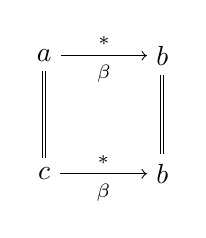
\begin{tikzpicture}[auto]
                \node (a) at (0,0) {$a$}; \node (b) at (1.5,0) {$b$};
                \node (c) at (0,-1.5) {$c$}; \node (b') at (1.5,-1.5) {$b$};
                \draw[->] (a) to node[above]{$\scriptstyle *$} (b);
                \draw[] (a) to node[below]{$\scriptstyle \beta$} (b);

                \draw[double] (a) to (c);

                \draw[double] (b) to (b');

                \draw[->] (c) to node[above]{$\scriptstyle *$} (b');
                \draw[] (c) to node[below]{$\scriptstyle \beta$} (b');

            \end{tikzpicture}
        \]
        \item If $n > 0$ then we have
            \[
                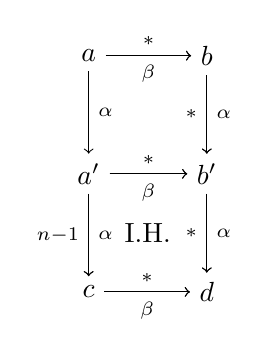
\begin{tikzpicture}[auto]
                \node (a) at (0,0) {$a$}; \node (b) at (1.5, 0) {$b$};
                \node (a') at (0, -1.5) {$a'$}; \node (b') at (1.5, -1.5) {$b'$};
                \node (c) at (0, -3) {$c$}; \node (d) at (1.5,-3) {$d$};
                \node (IH) at (0.75, -(1.5 + 0.75) {I.H.};

                \draw[->] (a) to node[above]{$\scriptstyle *$} (b);
                \draw[->] (a) to node[below]{$\scriptstyle \beta$} (b);
                
                \draw[->] (a) to node{$\scriptstyle \alpha$} (a');
                
                \draw[->] (a') to node[swap]{$\scriptstyle n-1$} (c);
                \draw[->] (a') to node{$\scriptstyle \alpha$} (c);

                \draw[->] (b) to node[swap]{$\scriptstyle *$} (b');
                \draw[->] (b) to node{$\scriptstyle \alpha$} (b');

                \draw[->] (b') to node[swap]{$\scriptstyle *$} (d);
                \draw[->] (b') to node{$\scriptstyle \alpha$} (d);

                \draw[->] (c) to node[above]{$\scriptstyle *$} (d);
                \draw[->] (c) to node[below]{$\scriptstyle \beta$} (d);

                \draw[->] (a') to node[above]{$\scriptstyle *$} (b');
                \draw[->] (a') to node[below]{$\scriptstyle \beta$} (b');
            \end{tikzpicture}
        \]
    \end{itemize}
\end{proof}

\section*{1.33 (b)}

%On whiteboard.

Let $\mathcal{A} = \langle \mathbb{N}, \{\to_1, \to_2\} \rangle$ be an ARS
    where $\to_1\; = \{(n, n+1) \mid n \in \mathbb{N}\}$ and $\to_2 \;= \{(n, n+2 \mid n \in \mathbb{N}\}$.

\begin{example}
    \[
    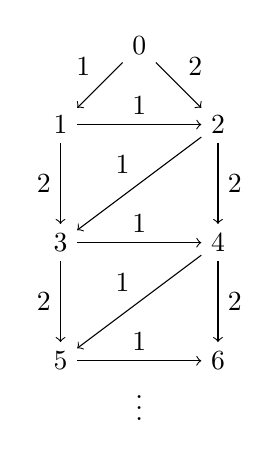
\begin{tikzpicture}[auto]
        \node (0) at (0,0) {$0$};
        \node (1) at (-1,-1) {$1$}; \node (2) at (1,-1) {$2$};
        \node (3) at (-1,-2.5) {$3$}; \node (4) at (1,-2.5) {$4$};
        \node (5) at (-1,-4) {$5$}; \node (6) at (1,-4) {$6$};
        %\node (7) at (-1,-5.5) {$7$}; \node (8) at (1,-5.5) {$8$};
        \node (vd1) at (0,-4.5) {$\vdots$};
        
        \draw[->] (0) to node[swap]{$1$} (1);
        \draw[->] (0) to node[]{$2$} (2);
        \draw[->] (1) to node[swap]{$2$} (3);
        \draw[->] (1) to node{$1$} (2);
        \draw[->] (2) to node{$2$} (4);
        \draw[->] (2) to node[swap]{$1$} (3);
        \draw[->] (3) to node{$1$} (4);
        \draw[->] (3) to node[swap]{$2$} (5);
        \draw[->] (4) to node{$2$} (6);
        \draw[->] (4) to node[swap]{$1$} (5);
        \draw[->] (5) to node{$1$} (6);
    \end{tikzpicture}
    \]
\end{example}

\begin{claim*}
    The ARS $\mathcal{A}$ is peak decreasing.
\end{claim*}

\begin{proof}
    Let $c$ $_2\!\leftarrow a \to_1 b$.
    According to the definition of $\to_1$ and $\to_2$, we have $b = a+1$ and $c = a+2$.
    So we have $c = b+1$. Thus $b \to_1 c$ holds.
    Since $2 > 1$, $c \xleftrightarrow[\vee 12]{*} b$ holds.
\end{proof}

\begin{claim*}
    The ARS is not connected.
\end{claim*}
\begin{proof}
    Take $1$ $_1\!\leftarrow 0 \to_2 2$. Then $1 \leftrightarrow^* 2$ but $0 \ngtr 1$.
\end{proof}

\section*{1.34 (b)}

\begin{claim*}
    Let $\mathcal{A} = \langle A, \{\alpha, \beta, \gamma\} \rangle$ be an ARS.
    If $\alpha/(\beta \cup \gamma)$ and $\beta/\gamma$ are terminating
    then $(\alpha \cup \beta) / \gamma$ is terminating.
\end{claim*}

\begin{proof}
    To prove the claim, we show that $\gamma^*(\alpha \cup \beta)$ is terminating.
    We distinguish two cases.
    \begin{itemize}
        \item If $\gamma^*\beta$ then it is terminating by the assumption.
        \item If $\gamma^*\alpha$ then suppose $\gamma^*\alpha$ is not terminating.
        Then $\alpha$ is not terminating. However since $\alpha/(\beta \cup \gamma)$ is terminating,
        $\alpha$ is terminating. Hence we have contradiction.
    \end{itemize}
\end{proof}

\end{document}
